\section{Implementation} \label{implementation}
This section explains the different protocols and algorithms OmniLedger uses, as well as how they were implemented.

\subsection{Sharding assignment} \label{sharding}
The sharding assignment algorithm takes as input a roster $R$ (i.e. list of nodes), a number of shard $n$ and an initial seed $s$. It starts by computing a random permutation of the nodes in $R$ using the given seed $s$. Then, it forms $n$ shards based on the previously computed random permutation. The algorithm is designed to compute a "fair" sharding assignment, i.e. the difference in size between any two shards is at most one. The algorithm has two main steps, the first is to slice the roster such that every shard has the same number of nodes, the second is to assign the remaining nodes uniformly. \\\\
$R$ should be the identity ledger roster, i.e. all nodes participating in the network. $n$ should be low enough such that the resulting shards have enough nodes to ensure some security properties: Omniledger employs ByzCoinX\cite{kokoris-kogias_enhancing_2016} as its consensus protocol, it provides consensus in a Byzantine setting as long as the number of malicious nodes is less than a third of the total number of validators. \\\\
A new sharding assignment is computed during an OmniLedger's creation and at the start of a new epoch. \\\\
As for the implementation, the sharding assignment is computed by a function, which is called in the OmniLedger Epoch contract when executing the \texttt{spawn:omniledgerepoch} or the \texttt{invoke:req\_new\_epoch} instruction. The implementation currently uses the hash of the received instruction as seed. This is not secure as an attacker could change the seed by modifying the instruction (instructions are signed with a Schnorr signature which employs a random component during the signature generation, as a result an attacker could sign the instruction multiple times until it obtains a seed to their liking). The solution would be to use a bias-resistant distributed randomness protocol, e.g. RandHound\cite{cryptoeprint:2016:1067}, as mentioned in the OmniLedger paper.

\begin{figure}
	\centering
	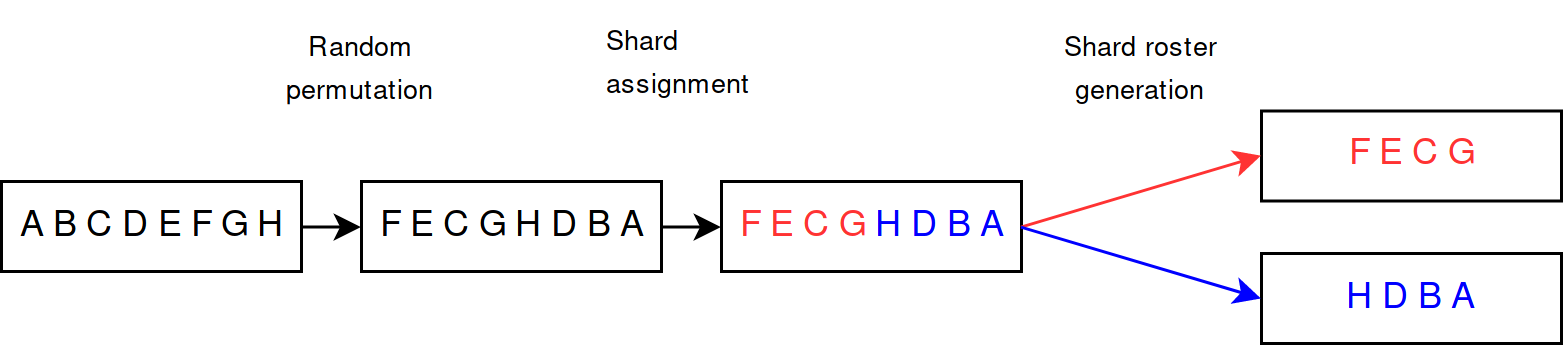
\includegraphics[width=\textwidth]{sharding1.png}
	\caption{\label{fig:sharding1} Example of a sharding assignment execution}
\end{figure}

\begin{figure}
	\centering
	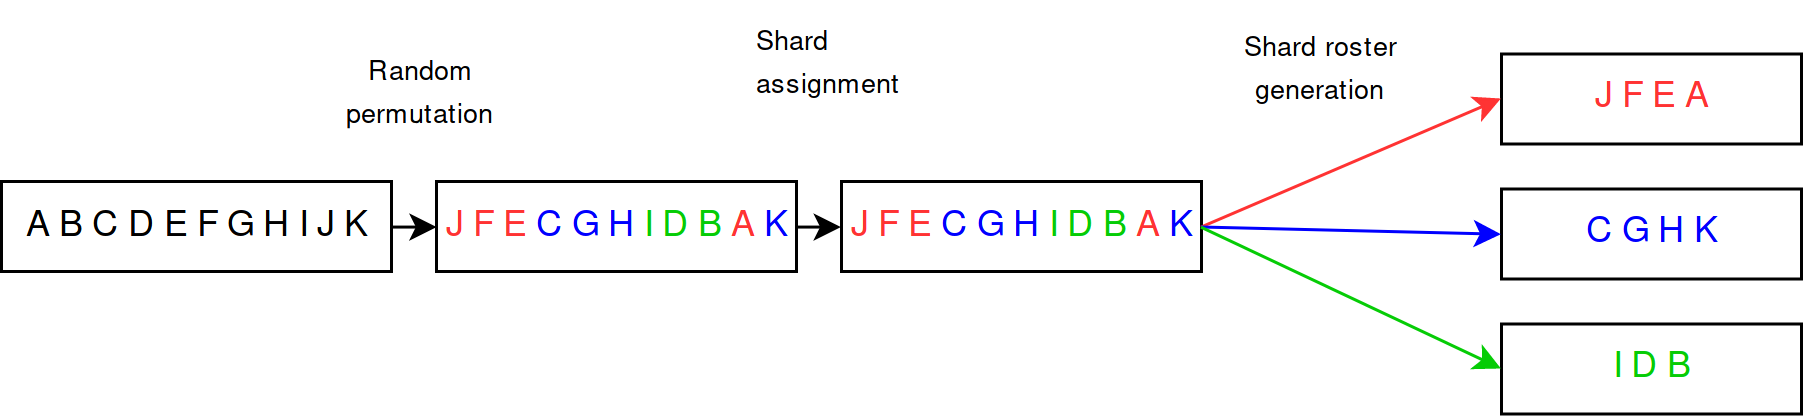
\includegraphics[width=\textwidth]{sharding2.png}
	\caption{\label{fig:sharding2} Another example of a sharding assignment execution where the concept of "fair" assignment is illustrated: nodes A and K are assigned to roster 1 and 2 respectively, instead of both being assigned to roster 1}
\end{figure}


\subsection{Applying roster change} \label{apply-roster-change}
Once a new sharding assignment has been computed, the changes must be communicated and applied to the shards. New shard rosters are applied shard-by-shard. To go from the current shard roster $R$ to the new shard roster $R'$, the algorithm always start by adding new nodes (i.e. $nodes$ such that $nodes \in R' \land  nodes \notin R$) and then removes old nodes (i.e. $nodes$ such that $nodes \notin R' \land nodes \in R$). One critical property of the algorithm is that it is designed to add or remove nodes one-by-one instead of in batches. This is done to ensure that shards will always have enough validators to keep processing transactions during the transition from old to new roster. \\\\
In terms of implementation, the application of roster change is part of the Config smart contract of ByzCoin, in particular, one can execute it by sending a transaction containing the \texttt{invoke:new\_epoch} instruction. The latter must contain as arguments a proof of the new epoch (obtained from requesting a new epoch from the IB) and the index of the shard to be updated. Upon receiving the instruction, the shard ledger starts by verifying the proof, if it's valid it decodes it to get the new roster. Then, it will fetch the current roster from the instance data. Finally, it computes the intermediate roster using the change roster function and update the current roster to the intermediate. Note that because changes are applied one at the time, the same transaction must be sent multiple times to the ledger in order to completely change the shard roster from old to new.  This implies the shard roster, and consequently also the instance data and the ledger state, will change gradually. \\\\
The examples below show how roster changes are computed. Notice that after the second call in the first example, the order in the returned roster changed, in particular new nodes were put in front of the roster. The algorithm puts new nodes in fron of the roster when all nodes have been added. The motivation behind such a change is to guarantee that the leader won't be removed (in ByzCoin, the first node in the roster list is considered the leader). Also notice that the examples employs two shards which do not meet the required number of validators (each should have at least 4 nodes) for the sake of brevity.
\begin{lstlisting}[basicstyle=\ttfamily\footnotesize]
cur = [A,B]; 
new = [C,D];
1st call: cur = ChangeRoster(curr, new); // cur is [A,B,C]
2nd call: cur = ChangeRoster(curr, new); // cur is [C,D,A,B]
3rd call: cur = ChangeRoster(curr, new); // cur is [C,D,B]
4th call: cur = ChangeRoster(curr, new); // cur is [C,D]
\end{lstlisting}

\begin{lstlisting}[basicstyle=\ttfamily\footnotesize]
cur = [A,B,C]; 
new = [C,D,E];
1st call: cur = ChangeRoster(curr, new); // cur is [A,B,C,D]
2nd call: cur = ChangeRoster(curr, new); // cur is [C,D,E,A,B]
3rd call: cur = ChangeRoster(curr, new); // cur is [C,D,E,B]
4th call: cur = ChangeRoster(curr, new); // cur is [C,D,E]
\end{lstlisting}

\subsection{Timestamps} \label{timestamp}
Timestamps are used in both the creation of a new OmniLedger and the request of a new epoch. The need for timestamps stems from one of the requirement in the new epoch protocol: to check if enough time has elapsed since the previous successful new epoch. Thus, the idea was to add a timestamp, computed on the client side, to user requests, and use it to determine the validity of the request, i.e. a new epoch request is valid if the difference in time between its timestamp $t_{req}$ an the previous new epoch's timestamp $t_{prev}$  is larger than the epoch size $es$ or $|t_{req} - t_{prev}| \geq es$. Consequently, request for the creation of a new OmniLedger also had to include a timestamp to mark the first successful epoch. \\\\
However, this came with some security issues: An attacker could manipulate $t_{req}$ by changing the internal clock of its machine before the client program computes it. To mitigate this problem, the OmniLedger Epoch contract includes an additional check: it verifies that $t_{req}$ is within some time window from the node's clock $nc$, i.e. $t_{req}$ is at most either $w$ seconds earlier or later than the node's clock for the request to be considered valid or $|t_{req} - nc| \leq w$. The value of $w$ is a parameter that is hard-coded at the moment (current value is 60 seconds), but one could refactor the code to make it an OmniLedger parameter.

\subsection{OmniLedger creation} \label{ol-creation}
The OmniLedger creation protocol is used to set up an new OmniLedger. It is composed of multiple steps from which include the creation of the IB, the initial sharding assignment, the creation of the shard ledgers and so on. Below is a detailed description of each steps.
\begin{enumerate}
	\item The protocol starts with the execution of the \texttt{create} command from the CLI client, it must provide as argument an initial list of participating nodes in a roster file, the number of shards and the epoch size. The client will construct and fill a request partially before sending it to the OmniLedger client. In particular, it computes and includes a timestamp in the request.
	
	\item The OmniLedger client takes care of creating the missing elements and filling the request before sending it to the OmniLedger service. The missing elements are: a new identity for the owner of the OmniLedger (contains the private/public key pair), a genesis message for the IB and the \texttt{spawn:omniledgerepoch} instruction. The latter will not be included in the request directly, instead a transaction containing the instruction will be created and added to the request. The transaction also need to be signed with the private key of the owner. The motivation for doing this operation on the OmniLedger client rather than on the service is to avoid sending the private key over the network, which is unsecure.
	
	\item Upon reception of the request message, the service starts with the creation of the IB ledger. This is done by contacting the ByzCoin service with the previously mentioned genesis message. Next, the service sends the transaction containing the \texttt{spawn:omniledgerepoch} instruction to the newly created IB. 
	
	\item As the IB receives the transaction, it first check that the request timestamp is not too different from the node's clock (see section \ref{timestamp}). Then, it computes sharding assignment using the roster provided in the transaction before saving the roster, the shard count, the epoch size, the timestamp and the shard rosters as instance data and return state changes. This whole step is part of the OmniLedger Epoch contract.
	
	\item Once the transaction is on the IB, the service can fetch the newly computed shard rosters. To do this, the service asks the IB for a proof that the spawn instruction was well executed. After verifying the proof, the service can decode it to get the instance data saved in the previous step, among which are the shard rosters. Now, the service can create the shard ledgers similarly to how the IB was created: for each shard, a genesis message contaning the corresponding shard roster is created, before being sent to the ByzCoin service to create the ledger.
	
	\item After the creation of the shard ledgers, the service can send a response to the CLI client. It includes the identity ledger's ID and roster, the shard ledgers' IDs and the OmniLedger Epoch instance ID. In addition, the key pair generated in the earlier steps is also returned to the CLI client.
	
	\item When the client receives the response, it saves the relevant information in a config file and the generated key pair in a key file.
\end{enumerate}
The appendix contains a diagram annotated with step numbers showing communication flows during the execution of the protocol. 

\subsection{New epoch} \label{new-epoch}
The new epoch protocol is used to request the start of a new epoch. It begins with the computation of a new sharding assignment before communicating the new rosters to the shard ledgers. A detailed description of each steps can be found below. 
\begin{enumerate}
	\item The protocol starts with the execution of the \texttt{newepoch} command from the CLI. The user must provide the  configuration file of the Omniledger it desires to speak to and the corresponding key file. The client will load both files and build a request. Once again, a timestamp is added before the request is sent to the service via an OmniLedger client.
	
	\item The OmniLedger client starts by preparing a transaction containing a \texttt{invoke:request\_new\_epoch} (signing the transaction, incrementing the signer counter) and sends it to the OmniLedger service.
	
	\item The OmniLedger service forwards the transaction to the IB ledger.
	
	\item The IB executes the code according to the OmniLedger Epoch contract: it starts by comparing the timestamp of the request with the node's timestamp to make sure they're not too different. Next, it fetches the instance data to get the current roster, as well as the epoch size and the timestamp marking the previous successful new epoch. Then, it computes the difference between between the request timestamp and the instance data timestamp and checks that it is larger than the epoch size. If this is the case, the IB can compute a new sharding assignment using the instruction's hash as seed, update the instance data with the new timestamp and roster before finally returning state changes.
	
	\item Once the new sharding assignment is completed, the OmniLedger service fetches the proof of the instruction and sends it back to the OmniLedger client as response.
	
	\item The OmniLedger client verifies and decodes the proof to get the new shard rosters. For each shard, the client creates and prepare a transaction with a \texttt{invoke:new\_epoch} instruction which contains the new roster. As described in section \ref{apply-roster-change}, this transaction must be sent multiple times (with a few changes such as incrementing the signer counter and re-signing) to the shard ledger until all changes are applied. The exact number of changes can be computed as the set difference between the old and new roster of the shard, i.e. the number of nodes present in the old roster but not in the new one.
	
	\item Once all roster are applied, the OmniLedger client can return the IB roster to the CLI client. The latter will save it in the configuration file.
\end{enumerate}
The appendix contains a diagram annotated with step numbers showing communication flows during the execution of the protocol. 

\subsection{Get status}
The get status protocol is used to learn about the current rosters (IB and shard) of an OmniLedger. Its steps are described below. 
\begin{enumerate}
	\item The protocol starts with the execution of the \texttt{status} command from the CLI. The command takes as parameter the configuration file of the OmniLedger the user desires to speak with. The configuration file holds, among other things, the identity of the OmniLedger's IB and the identity of the instance containing the rosters information. The CLI client will create and fill the request, then send it to the OmniLedger client. 
	
	\item The OmniLedger client sends the request directly to the ByzCoin service via a Byzcoin client. 
	
	 \item The OmniLedger client obtains a reponse containing a proof to verify and decode from the BC service. 
	 
	 \item After decoding the proof, it creates and fills a response message with the current IB roster and shard rosters, then sends it to the CLI client. 
	
	\item The CLI client can output the current roster and shard rosters.
\end{enumerate}
The appendix contains a diagram annotated with step numbers showing communication flows during the execution of the protocol. 

\subsection{Testing}
In addition to the implementation code, automatic tests were written. There are two types of test in this project: Unit tests and integration tests. \\\\
Unit tests were written in Go using a mix of the built-in package \texttt{testing}\cite{testing}, ONet's local testing framework\cite{onet}, and the \texttt{Testify}\cite{testify} library. They test the more important functions such as new roster computation or the application of roster changes. To run unit tests, execute the Go command \texttt{go test} in the relevant directory. An individual test can also be run by using the command \texttt{go test -run <Name of test>}. \\\\
Integration tests are written as shell scripts and use ONet's specialised testing bash-library\cite{libtest}. They aim to validate the integration and interaction of the different components, from the CLI-client call to the contract execution. In particular, tests were written for new Omniledger creation, new epoch request and status request. To run the integration tests, execute the shell script \texttt{omniledger/oladmin/test.sh}. In its current state, shard assignment has only been tested on a local machine with 8 conodes.

\subsection{Documentation}
In order to facilitate code understanding and code re-use, public functions and structures were documented with comments. This is also the case for important private functions.
